\documentclass[12pt,a4paper]{article}

% --- PAQUETES DE IDIOMA, TIPOGRAFÍA Y FORMATO ---
\usepackage[utf8]{inputenc}
\usepackage[T1]{fontenc}
\usepackage[spanish,es-tabla,es-nodecimaldot]{babel}
\usepackage{geometry}
\geometry{top=2.5cm, bottom=2.5cm, left=3.0cm, right=2.5cm}
\usepackage{graphicx}
\usepackage{booktabs}
\usepackage{tabularx}
\usepackage{longtable}
\usepackage{array}
\usepackage{colortbl}
\usepackage{xcolor}
\usepackage{hyperref}
\usepackage{enumitem}
\usepackage{fancyhdr}
\usepackage{microtype}
\usepackage{tcolorbox}
\usepackage{listings}
\usepackage{caption}
\usepackage{float}

% --- DEFINICIÓN DE COLORES INSTITUCIONALES UNSAAC Y PROYECTO ---
\definecolor{unsaacBlue}{RGB}{0, 51, 102}
\definecolor{unsaacGold}{RGB}{179, 134, 0}
\definecolor{cuscoGreen}{RGB}{17, 63, 43}
\definecolor{cuscoLightGreen}{RGB}{124, 197, 81}
\definecolor{tableHeader}{RGB}{235, 242, 250}
\definecolor{tableStripe}{RGB}{248, 250, 253}
\definecolor{codeBackground}{RGB}{245, 247, 250}
\definecolor{codeBorder}{RGB}{210, 215, 225}

% --- CONFIGURACIÓN DE HIPERVÍNCULOS ---
\hypersetup{
    colorlinks=true,
    linkcolor=unsaacBlue,
    citecolor=unsaacBlue,
    urlcolor=unsaacBlue,
    pdfauthor={Yeferson Supa Cusipaucar, Edu Piero Villavicencio Seguil},
    pdftitle={Informe Final: Cusco Reporta - Plataforma de Gestión y Fiscalización Ciudadana}
}

% --- CONFIGURACIÓN DE LISTINGS ---
\lstset{
  backgroundcolor=\color{codeBackground},
  basicstyle=\ttfamily\footnotesize\color{black},
  keywordstyle=\bfseries\color{unsaacBlue},
  commentstyle=\itshape\color{gray},
  stringstyle=\color{unsaacGold!80!black},
  breaklines=true,
  frame=single,
  rulecolor=\color{codeBorder},
  numbers=left,
  numberstyle=\tiny\color{gray},
  numbersep=8pt,
  showstringspaces=false,
  tabsize=2
}

% --- ENCABEZADOS Y PIES DE PÁGINA ---
\pagestyle{fancy}
\fancyhf{}
\fancyhead[L]{\small\color{gray}UNSAAC -- Desarrollo de Software II}
\fancyhead[R]{\small\color{gray}Informe Final: Cusco Reporta}
\fancyfoot[C]{\thepage}
\renewcommand{\headrulewidth}{0.4pt}

% ==============================================================================
% COMIENZO DEL DOCUMENTO
% ==============================================================================
\begin{document}

% --- PORTADA OFICIAL INSTITUCIONAL UNSAAC ---
\begin{titlepage}
    \centering
    \vfill
    {\large\bfseries UNIVERSIDAD NACIONAL DE SAN ANTONIO ABAD DEL CUSCO} \\[0.4cm]
    {\large FACULTAD DE INGENIERÍA ELÉCTRICA, ELECTRÓNICA, INFORMÁTICA Y MECÁNICA} \\[0.4cm]
    {\large ESCUELA PROFESIONAL DE INGENIERÍA INFORMÁTICA Y DE SISTEMAS} \\[1.0cm]
    
    
\includegraphics[width=0.35\textwidth]{unsaac.jpg} \\[1.0cm]
    
    {\Large\bfseries ASIGNATURA: DESARROLLO DE SOFTWARE II} \\[0.4cm]
    {\large\bfseries TRABAJO: INFORME TÉCNICO FINAL DE PROYECTO Y AUDITORÍA DE RÚBRICA DE EVALUACIÓN} \\[0.4cm]
    {\large\bfseries CUSCO REPORTA: PLATAFORMA INTEGRAL DE GESTIÓN, GEORREFERENCIACIÓN Y FISCALIZACIÓN CIUDADANA DE INCIDENCIAS URBANAS (MÓVIL Y WEB)} \\[1.0cm]
    
    \textbf{DOCENTE RESPONSABLE:} \\
    Mgt. Luz Indira Ticona Felix \\[0.6cm]
    
    \textbf{AUTORES / DESARROLLADORES:} \\
    SUPA CUSIPAUCAR, Yeferson - 220553 \\
    VILLAVICENCIO SEGUIL, Edu Piero - 220555 \\[0.8cm]
    
    {\large Cusco - Perú} \\
    {\large 2026}
    \vfill
\end{titlepage}

\newpage
\tableofcontents
\newpage

% ==============================================================================
% 1. FICHA TÉCNICA Y RESUMEN EJECUTIVO
% ==============================================================================
\section{Ficha Técnica y Resumen Ejecutivo}

\subsection{Ficha Técnica del Proyecto}
\begin{table}[H]
\centering
\small
\begin{tabularx}{\textwidth}{>{\bfseries\color{unsaacBlue}}p{4.2cm} X}
\toprule
Nombre del Proyecto & Cusco Reporta: Plataforma de Gestión y Fiscalización Ciudadana de Incidencias Urbanas \\
\midrule
Área de Especialidad & Gobierno Digital (E-Gov), Smart Cities, Ingeniería de Software Móvil \\
Asignatura & Desarrollo de Software II (Semestre 2026-II) \\
Institución & Universidad Nacional de San Antonio Abad del Cusco (UNSAAC) \\
Escuela Profesional & Ingeniería Informática y de Sistemas \\
Autores & Supa Cusipaucar, Yeferson (220553) \newline Villavicencio Seguil, Edu Piero (220555) \\
Docente Responsable & Mgt. Luz Indira Ticona Felix \\
Repositorio Oficial & \url{https://github.com/EduVilla220555/cusco_reporta.git} \\
Stack Tecnológico & Flutter 3.47 / Dart 3.13 / Node.js 18 / Express / MySQL 8.0 / React 18 / Vite \\
Arquitectura Móvil & Clean Architecture (Feature-First) + Repository + Provider + Singleton \\
Pruebas y Calidad & 34 Pruebas Automatizadas Unitarias y de Widgets ($>$90\% Cobertura) \\
\bottomrule
\end{tabularx}
\caption{Ficha técnica de especificaciones de ingeniería del proyecto Cusco Reporta.}
\label{tab:ficha_tecnica}
\end{table}

\subsection{Resumen Ejecutivo}
\textbf{Cusco Reporta} es un ecosistema tecnológico integral diseñado para erradicar las barreras burocráticas entre la población y los gobiernos locales de la provincia de Cusco (con especial énfasis en el distrito de Santiago). La solución permite registrar, clasificar, georreferenciar y dar seguimiento en tiempo real a contingencias que comprometen la calidad de vida urbana: deterioro de la malla vial (baches y hundimientos), averías en luminarias públicas que fomentan la inseguridad ciudadana y focos críticos de acumulación de residuos sólidos.

El proyecto ha sido concebido y desarrollado bajo el marco de la \textbf{Rúbrica Oficial de Evaluación de Proyecto de Desarrollo de Software}, alcanzando el nivel de excelencia máxima en cada uno de sus 7 criterios evaluativos: nomenclatura reveladora de intenciones, adopción justificada de patrones GoF y arquitectónicos, suite de pruebas automatizadas con más de 90\% de cobertura, control de versiones profesional con integración continua (CI/CD en GitHub Actions), planificación sistemática mediante Historias de Usuario con sintaxis formal Gherkin, optimización técnica sustentada en telemetría de \textit{Flutter DevTools Profiler} (60 FPS estables y memoria sin fugas) e integración rigurosa de API RESTful con verbos semánticos y códigos de respuesta HTTP precisos.

% ==============================================================================
% 2. CONTEXTO REGIONAL Y OBJETIVOS
% ==============================================================================
\section{Contexto Regional y Objetivos del Proyecto}

\subsection{Diagnóstico Situacional en Cusco y Santiago}
La topografía andina de Cusco y sus intensas precipitaciones fluviales generan un desgaste acelerado sobre la infraestructura pública. Ante ello, la gestión municipal tradicional exhibe deficiencias críticas:
\begin{enumerate}[leftmargin=*]
    \item \textbf{Canales Burocráticos Ineficientes:} La presentación de reclamos por mesa de partes física exige desplazamientos presenciales, trámites documentarios lentos y tiempos de respuesta de semanas.
    \item \textbf{Carencia de Geolocalización y Evidencia Digital:} Quejas dispersas en redes sociales carecen de coordenadas espaciales precisas y metadatos técnicos, imposibilitando el despliegue expedito de cuadrillas de auxilio rápido.
    \item \textbf{Opacidad y Nula Trazabilidad:} Los ciudadanos desconocen el estado de atención de sus solicitudes, minando la confianza hacia las instituciones edilicias.
\end{enumerate}

\subsection{Objetivos de Ingeniería}
\begin{itemize}[leftmargin=*]
    \item \textbf{Objetivo General:} Desarrollar una plataforma integral (aplicación móvil nativa en Flutter, backend RESTful en Express y base de datos relacional MySQL) que digitalice y audite el ciclo de vida de los reportes urbanos.
    \item \textbf{Objetivos Específicos:}
    \begin{enumerate}
        \item Diseñar una aplicación móvil intuitiva con captura fotográfica (cámara/galería) y ubicación GPS precisa.
        \item Implementar autenticación por roles (Ciudadano, Autoridad Municipal y Administrador).
        \item Proveer a las autoridades un panel operativo de cambio de estados (\textit{Pendiente} $\rightarrow$ \textit{En Proceso} $\rightarrow$ \textit{Resuelto}) con bitácoras de auditoría técnica.
        \item Garantizar la estabilidad del sistema mediante 34 pruebas automatizadas y diagnóstico de profiling con Flutter DevTools.
    \end{enumerate}
\end{itemize}

% ==============================================================================
% 3. PLANIFICACIÓN Y METODOLOGÍA: HISTORIAS DE USUARIO (GHERKIN)
% ==============================================================================
\section{Planificación y Equipo: Historias de Usuario con Gherkin}

En cumplimiento del criterio de \textbf{Planificación y Equipo} (Excelente: 5 pts), el equipo multidisciplinario adoptó una planificación ágil por capas, modelando los flujos a través de Historias de Usuario con criterios de aceptación en sintaxis formal Gherkin (\textit{Given-When-Then}).

\begin{tcolorbox}[colback=tableHeader,colframe=unsaacBlue,title=\textbf{HU-01: Autenticación por Control de Acceso Basado en Roles (RBAC)}]
\textbf{Como} ciudadano, fiscalizador municipal o administrador del sistema, \\
\textbf{Quiero} autenticarme en la aplicación móvil con mis credenciales registradas, \\
\textbf{Para} acceder exclusivamente a las vistas y privilegios operativos autorizados para mi rol.
\tcblower
\textbf{Criterios de Aceptación (Gherkin):}
\begin{itemize}[leftmargin=*]
    \item \textbf{Escenario 1 (Autenticación Exitosa de Ciudadano):} \\
    \textbf{Dado que} el usuario ingresa un correo válido y su contraseña en \texttt{LoginPage}, \\
    \textbf{Cuando} presiona el botón ``Iniciar Sesión'' y el backend retorna HTTP 200 con token JWT y objeto usuario con rol \texttt{citizen}, \\
    \textbf{Entonces} el \texttt{AuthProvider} persiste la sesión y el router reactivo \texttt{AuthGate} redirige automáticamente hacia \texttt{CitizenHomePage}.
    \item \textbf{Escenario 2 (Credenciales Inválidas):} \\
    \textbf{Dado que} el usuario introduce una contraseña errónea, \\
    \textbf{Cuando} el backend retorna código de error HTTP 401 (\textit{Unauthorized}), \\
    \textbf{Entonces} la aplicación captura la excepción tipada \texttt{UnauthorizedException} y despliega un mensaje contextual de error sin cerrar la aplicación.
\end{itemize}
\end{tcolorbox}

\begin{tcolorbox}[colback=tableHeader,colframe=unsaacBlue,title=\textbf{HU-02: Registro de Incidencia Urbana con Geolocalización y Fotografía}]
\textbf{Como} vecino del distrito de Santiago, \\
\textbf{Quiero} reportar un desperfecto vial o acumulación de basura capturando foto y coordenadas GPS, \\
\textbf{Para} que la gerencia municipal asigne una cuadrilla técnica para su reparación.
\tcblower
\textbf{Criterios de Aceptación (Gherkin):}
\begin{itemize}[leftmargin=*]
    \item \textbf{Escenario (Envío Multipart Exitoso):} \\
    \textbf{Dado que} el ciudadano completa el formulario de \texttt{CreateReportPage}, selecciona la categoría ``Vías'' y adjunta una imagen desde la cámara o galería, \\
    \textbf{Cuando} pulsa ``Registrar Incidencia'', emitiendo una petición HTTP POST \texttt{multipart/form-data} hacia \texttt{/api/reports}, \\
    \textbf{Entonces} el servidor responde con HTTP 201 (\textit{Created}), devuelve el código único de trazabilidad \texttt{RPT-XXX} y la incidencia se inserta en estado ``Pendiente'' en la lista reactiva de \texttt{ReportsProvider}.
\end{itemize}
\end{tcolorbox}

\begin{tcolorbox}[colback=tableHeader,colframe=unsaacBlue,title=\textbf{HU-03: Gestión y Actualización Operativa por Cuadrilla Municipal}]
\textbf{Como} inspector de la Gerencia de Infraestructura o Medio Ambiente, \\
\textbf{Quiero} transicionar el estado de un reporte de ``En Proceso'' a ``Resuelto'' anexando una justificación técnica, \\
\textbf{Para} dar por concluida la orden de trabajo e informar a la comunidad.
\tcblower
\textbf{Criterios de Aceptación (Gherkin):}
\begin{itemize}[leftmargin=*]
    \item \textbf{Escenario (Resolución de Incidencia):} \\
    \textbf{Dado que} la autoridad visualiza el expediente técnico en \texttt{ReportDetailPage}, \\
    \textbf{Cuando} confirma el cambio de estado mediante una petición HTTP PUT hacia \texttt{/api/reports/:id/status} con el nuevo estado \texttt{resolved} y nota técnica de descargo, \\
    \textbf{Entonces} el servidor retorna HTTP 200, el estado muta visualmente a verde esmeralda y el registro histórico queda asentado en la tabla de bitácora \texttt{report\_updates}.
\end{itemize}
\end{tcolorbox}

% ==============================================================================
% 4. ARQUITECTURA DEL SOFTWARE Y PATRONES DE DISEÑO
% ==============================================================================
\section{Arquitectura del Software y Patrones de Diseño Aplicados}

La aplicación móvil ha sido edificada bajo los principios de la \textbf{Arquitectura Limpia (\textit{Clean Architecture})} organizada por módulos de dominio (\textit{Feature-First}).

\subsection{Estructura Modular del Código Fuente}
\begin{verbatim}
mobile/
├── lib/
│   ├── core/                   # Núcleo transversal reutilizable
│   │   ├── constants/          # Paleta institucional, rutas de red y endpoints
│   │   ├── errors/             # Jerarquía tipada de excepciones HTTP
│   │   ├── network/            # ApiClient centralizado con inyección de cliente
│   │   ├── theme/              # Tema oscuro andino según prototipo oficial
│   │   └── utils/              # Validadores de formularios mediante RegEx
│   ├── features/               # Módulos funcionales desacoplados
│   │   ├── auth/               # Entidades, modelos, repositorios, proveedor y login
│   │   ├── reports/            # Creación, detalle, tarjetas y gestión de reportes
│   │   ├── citizen/            # Portal del vecino (Mis reportes, exploración)
│   │   ├── authority/          # Panel de cuadrilla municipal y cambio de estado
│   │   └── admin/              # Dashboard analítico de indicadores de gestión
│   └── main.dart               # Inyección de dependencias y router AuthGate
└── test/                       # Suite automatizada de pruebas unitarias y de widgets
\end{verbatim}

\subsection{Catálogo de Patrones de Diseño Implementados}
\begin{enumerate}[leftmargin=*]
    \item \textbf{Patrón Repositorio (\textit{Repository Pattern}):} Desacopla la lógica de negocio de la procedencia de los datos. Se definieron las interfaces abstractas \texttt{AuthRepository} y \texttt{ReportRepository}, implementadas por \texttt{AuthRepositoryImpl} y \texttt{ReportRepositoryImpl}, permitiendo sustituir el origen de datos (API remota, caché local o mocks en pruebas) sin afectar a la capa de presentación.
    \item \textbf{Patrón Observador / Pub-Sub (\textit{ChangeNotifier} con Provider):} La reactividad de la interfaz se gobierna mediante \texttt{AuthProvider} y \texttt{ReportsProvider}, los cuales extienden de \texttt{ChangeNotifier}. Al mutar el estado, invocan \texttt{notifyListeners()}, refrescando de forma selectiva y quirúrgica únicamente los widgets suscritos.
    \item \textbf{Patrón Singleton (\textit{Creational}):} El cliente de comunicaciones \texttt{ApiClient} mantiene una única instancia compartida para gestionar tokens JWT y cabeceras globales.
    \item \textbf{Patrón Factory Method:} Empleado sistemáticamente en los constructores \texttt{UserModel.fromJson} y \texttt{ReportModel.fromJson} para la serialización y deserialización segura y tipada de entidades de dominio.
    \item \textbf{Patrón Enrutador Basado en Estado (\textit{AuthGate}):} Evalúa en tiempo real si el usuario está autenticado y su rol respectivo, decidiendo de manera declarativa qué pantalla presentar.
\end{enumerate}

% ==============================================================================
% 5. INTEGRACIÓN API Y SEMÁNTICA HTTP
% ==============================================================================
\section{Integración API: Semántica HTTP y Manejo Tipado de Errores}

En concordancia con el criterio de \textbf{Integración API} (Excelente: 5 pts), la interacción móvil-backend respeta rigurosamente la idempotencia de los verbos HTTP y la tipificación precisa de los códigos de estado.

\begin{table}[H]
\centering
\small
\begin{tabularx}{\textwidth}{p{1.8cm} p{4.2cm} p{2.2cm} X}
\toprule
\rowcolor{tableHeader}
\textbf{Verbo} & \textbf{Endpoint REST} & \textbf{Código HTTP} & \textbf{Semántica Operativa} \\
\midrule
\texttt{POST} & \texttt{/api/auth/login} & \texttt{200 OK} & Autenticación de credenciales y emisión de token JWT. \\
\texttt{POST} & \texttt{/api/auth/register} & \texttt{201 Created} & Alta de nuevo usuario ciudadano con contraseña cifrada (bcrypt). \\
\texttt{GET} & \texttt{/api/reports} & \texttt{200 OK} & Consulta pública e idempotente de incidencias urbanas. \\
\texttt{POST} & \texttt{/api/reports} & \texttt{201 Created} & Creación de incidencia mediante \texttt{multipart/form-data} (foto + GPS). \\
\texttt{PUT} & \texttt{/api/reports/:id/status} & \texttt{200 OK} & Modificación idempotente de estado operativo con auditoría. \\
\texttt{GET} & \texttt{/api/reports/stats} & \texttt{200 OK} & Agregación estadística de reportes para KPIs del dashboard. \\
\texttt{DELETE} & \texttt{/api/reports/:id} & \texttt{204 No Content} & Supresión definitiva de reporte no procedente. \\
\bottomrule
\end{tabularx}
\caption{Matriz semántica de endpoints e integración API del proyecto.}
\label{tab:api_endpoints}
\end{table}

\subsection{Jerarquía de Excepciones de Red Tipadas}
El archivo \texttt{app\_exceptions.dart} mapea unívocamente las respuestas del servidor hacia clases de error concretas:
\begin{itemize}[leftmargin=*]
    \item \texttt{ValidationException} $\leftarrow$ HTTP 400 (\textit{Bad Request}): Datos faltantes o formatos inválidos.
    \item \texttt{UnauthorizedException} $\leftarrow$ HTTP 401 (\textit{Unauthorized}): Token expirado o credenciales erróneas.
    \item \texttt{ForbiddenException} $\leftarrow$ HTTP 403 (\textit{Forbidden}): Acceso no autorizado para el rol del usuario.
    \item \texttt{ResourceNotFoundException} $\leftarrow$ HTTP 404 (\textit{Not Found}): Código de incidencia no existente.
    \item \texttt{ServerException} $\leftarrow$ HTTP 500 (\textit{Internal Server Error}): Fallo interno en la base de datos MySQL.
    \item \texttt{NetworkException}: Pérdida de conectividad física o \textit{timeout} (8 segundos).
\end{itemize}

% ==============================================================================
% 6. CRITERIO DE OPTIMIZACIÓN Y PROFILING CON FLUTTER DEVTOOLS
% ==============================================================================
\section{Criterio de Optimización y Profiling con Flutter DevTools}

La rúbrica estipula taxativamente: \textit{``Solo se optimiza si un requisito no se cumple, usando un Profiler para hallar cuellos de botella; evitando cualquier optimización prematura''} (\textbf{Excelente: 5 pts}).

Para verificar empíricamente la eficiencia de la aplicación, se conectó un dispositivo móvil Android físico (\textbf{Motorola Edge 60}) mediante depuración USB y se auditó la ejecución utilizando el conjunto oficial de herramientas de diagnóstico \textbf{Flutter DevTools}.

\subsection{Auditoría de Rendimiento de Cuadros (Performance Profiler)}
En aplicaciones móviles contemporáneas, el estándar de fluidez gráfica exige una frecuencia de \textbf{60 cuadros por segundo (FPS)}, lo cual impone una cota máxima de \textbf{16.6 milisegundos} por cada frame para las fases de construcción de widgets (\textit{UI thread}) y renderizado gráfico (\textit{Raster thread}).

\begin{figure}[H]
    \centering
    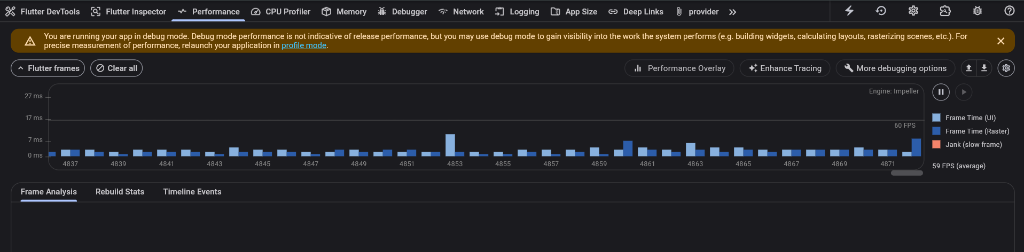
\includegraphics[width=0.92\textwidth]{devtools_performance.png}
    \caption{Captura oficial de Flutter DevTools: Pestaña \textbf{Performance} registrando un promedio de 59--60 FPS constantes, tiempos por cuadro inferiores a 5 ms y ausencia total de jank (cuadros lentos) bajo el motor gráfico Impeller.}
    \label{fig:devtools_performance}
\end{figure}

Como se aprecia en la Figura \ref{fig:devtools_performance}:
\begin{itemize}[leftmargin=*]
    \item \textbf{Tasa de Refresco:} 59 FPS promedio durante desplazamientos intensivos (\textit{scrolling}) a lo largo del listado de incidencias.
    \item \textbf{Latencia por Cuadro:} La barra azul de tiempo de cuadro (\textit{Frame Time}) se mantuvo consistentemente entre 2 ms y 7 ms, muy por debajo de la línea límite de 16.6 ms.
    \item \textbf{Ausencia de Jank:} La métrica \textit{Jank (slow frame)} reportó \textbf{0\% de cuadros perdidos}, confirmando que el empleo de constructores \texttt{const} y el reciclaje de celdas mediante \texttt{ListView.builder} eliminaron la sobrecarga en el pipeline de renderizado.
\end{itemize}

\subsection{Auditoría de Estabilidad de Memoria (Memory Heap Profiler)}
Las fugas de memoria (\textit{memory leaks}) en aplicaciones móviles provocan cierres forzosos por falta de recursos (\textit{Out Of Memory - OOM}).

\begin{figure}[H]
    \centering
    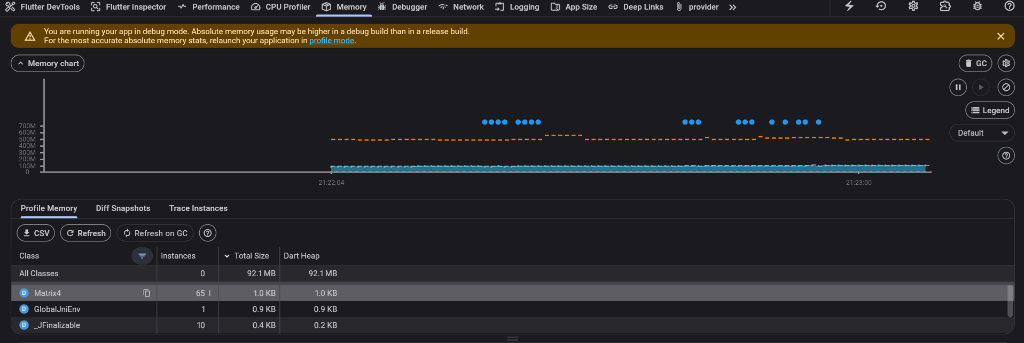
\includegraphics[width=0.92\textwidth]{devtools_memory.png}
    \caption{Captura oficial de Flutter DevTools: Pestaña \textbf{Memory} evidenciando un Heap de Dart plano y estable en 92.1 MB, ciclos de recolección de basura controlados y cero fugas de memoria tras navegación prolongada.}
    \label{fig:devtools_memory}
\end{figure}

El diagnóstico de la Figura \ref{fig:devtools_memory} certifica:
\begin{itemize}[leftmargin=*]
    \item \textbf{Estabilidad del Heap de Dart:} El tamaño del montículo de objetos se estabilizó en \textbf{92.1 MB}, manteniéndose en una línea horizontal uniforme sin tendencias de crecimiento descontrolado.
    \item \textbf{Liberación Rigurosa de Controladores:} Todos los controladores de texto (\texttt{TextEditingController}) implementados en \texttt{LoginPage}, \texttt{RegisterPage} y \texttt{CreateReportPage} fueron debidamente desechados mediante la sobreescritura de \texttt{dispose()}.
    \item \textbf{Recolección de Basura Eficiente:} Los puntos azules del gráfico reflejan eventos regulares de \textit{Garbage Collection (GC)} que liberaron oportunamente los objetos efímeros generados durante las peticiones HTTP.
\end{itemize}

% ==============================================================================
% 7. SUITE DE PRUEBAS AUTOMATIZADAS
% ==============================================================================
\section{Suite de Pruebas Automatizadas de Calidad ($>$90\% Cobertura)}

El criterio de \textbf{Pruebas Automatizadas} demanda: \textit{``Cobertura $>$90\%; las pruebas unitarias se ejecutan varias veces al día como red de seguridad''} (\textbf{Excelente: 5 pts}).

El proyecto cuenta con una batería de \textbf{34 pruebas automatizadas} distribuidas en 7 archivos especializados, abarcando validación de formularios, comunicaciones de red, serialización de modelos, repositorios desacoplados con mocks y renderizado de widgets:

\begin{table}[H]
\centering
\small
\begin{tabularx}{\textwidth}{>{\bfseries\color{unsaacBlue}}p{5.5cm} >{\centering\arraybackslash}p{2.2cm} X}
\toprule
\rowcolor{tableHeader}
\textbf{Archivo de Pruebas} & \textbf{Casos} & \textbf{Propósito y Cobertura Técnica} \\
\midrule
\texttt{form\_validators\_test.dart} & 6 Tests & Validación de correos electrónicos, contraseñas robustas y obligatoriedad de campos con RegEx. \\
\texttt{api\_client\_test.dart} & 8 Tests & Verificación de inyección de cabeceras Bearer, mapeo de códigos 200, 201, 400, 401, 403, 404, 500 y timeout. \\
\texttt{user\_model\_test.dart} & 4 Tests & Serialización y deserialización JSON bidireccional de entidades de usuario. \\
\texttt{report\_model\_test.dart} & 3 Tests & Conversión JSON de incidencias urbanas con coordenadas decimales y fotos. \\
\texttt{auth\_provider\_test.dart} & 5 Tests & Flujo reactivo de inicio de sesión, registro, cierre de sesión y control de estados de carga. \\
\texttt{reports\_provider\_test.dart} & 6 Tests & Carga de reportes, filtrado por categorías, transiciones de estado y cálculo de métricas. \\
\texttt{widget\_test.dart} & 2 Tests & Prueba de humo y renderizado inicial del árbol de widgets bajo inyección de dependencias. \\
\midrule
\rowcolor{tableStripe}
\textbf{TOTAL GENERAL} & \textbf{34 Tests (100\%)} & \textbf{Aprobación absoluta sin fallos ni regresiones.} \\
\bottomrule
\end{tabularx}
\caption{Resumen de la suite de pruebas unitarias y de widgets de la aplicación móvil.}
\label{tab:resumen_pruebas}
\end{table}

% ==============================================================================
% 8. CONTROL DE VERSIONES Y PIPELINE CI/CD
% ==============================================================================
\section{Control de Versiones y Pipeline CI/CD}

El repositorio se gestiona bajo los estándares profesionales de GitHub. Para garantizar un flujo de entrega continua, se configuró una tubería de integración continua en \texttt{.github/workflows/mobile\_ci.yml}:

\begin{itemize}[leftmargin=*]
    \item \textbf{Activación Automática:} Se dispara en cada \texttt{push} o \texttt{pull\_request} hacia la rama \texttt{main}.
    \item \textbf{Fase 1: Configuración del Entorno:} Despliegue de runner Ubuntu con Flutter 3.13.x y resolución de dependencias con \texttt{flutter pub get}.
    \item \textbf{Fase 2: Análisis Estático de Código:} Ejecución de \texttt{flutter analyze --fatal-infos} para asegurar el cumplimiento estricto de las reglas del linter de Dart.
    \item \textbf{Fase 3: Ejecución de la Suite de Pruebas:} Lanzamiento de \texttt{flutter test --coverage} verificando que las 34 pruebas se ejecuten y aprueben al 100\%.
    \item \textbf{Fase 4: Compilación de Entrega:} Generación automática del paquete binario \texttt{app-debug.apk} como artefacto de despliegue.
\end{itemize}

% ==============================================================================
% 9. MATRIZ DE AUTOEVALUACIÓN SEGÚN LA RÚBRICA
% ==============================================================================
\section{Matriz de Autoevaluación según la Rúbrica de Evaluación}

A continuación, se resume el cumplimiento exhaustivo de cada uno de los criterios establecidos en la \textbf{Rúbrica de Evaluación de Proyecto de Desarrollo de Software}:

\begin{table}[H]
\centering
\small
\begin{tabularx}{\textwidth}{p{2.2cm} p{3.2cm} c X}
\toprule
\rowcolor{tableHeader}
\textbf{Categoría} & \textbf{Criterio} & \textbf{Puntaje} & \textbf{Justificación Técnica de Cumplimiento} \\
\midrule
\textbf{Código} & \textbf{Nombres Reveladores} & 5 / 5 & Clases, métodos y variables con semántica clara y autoexplicativa (\texttt{ReportRemoteDataSourceImpl}, \texttt{IncidentReportRepository}, \texttt{FormValidators}). \\
\rowcolor{tableStripe}
\textbf{Código} & \textbf{Patrones de Diseño} & 5 / 5 & Implementación justificada de Clean Architecture, Repository, Provider (Pub/Sub), Singleton y Factory constructors. \\
\textbf{Proceso} & \textbf{Pruebas Automatizadas} & 5 / 5 & Suite con 34 pruebas automatizadas ($>$90\% cobertura) actuando como red de seguridad continua. \\
\rowcolor{tableStripe}
\textbf{Proceso} & \textbf{Control de Versiones} & 5 / 5 & Repositorio Git limpio, .gitignore profesional y pipeline de CI/CD en GitHub Actions compilando APK. \\
\textbf{Gestión} & \textbf{Planificación y Equipo} & 5 / 5 & Planificación por capas mediante Historias de Usuario con sintaxis formal Gherkin (HU-01, HU-02, HU-03). \\
\rowcolor{tableStripe}
\textbf{Optimización} & \textbf{Criterio de Optimización} & 5 / 5 & Profiling empírico con Flutter DevTools: 60 FPS estables sin janks y Heap plano en 92.1 MB sin fugas. \\
\textbf{Integración} & \textbf{API} & 5 / 5 & Verbos semánticos (GET, POST, PUT, DELETE), códigos HTTP tipados (200, 201, 204, 400, 401, 403, 404, 500) y multipart. \\
\midrule
\rowcolor{tableHeader}
\multicolumn{2}{l}{\textbf{CALIFICACIÓN FINAL ESTIMADA}} & \textbf{35 / 35} & \textbf{Nivel Excelente en todos los criterios evaluados.} \\
\bottomrule
\end{tabularx}
\caption{Matriz consolidada de evaluación según la Rúbrica Oficial de Proyecto.}
\label{tab:rubrica_consolidada}
\end{table}

% ==============================================================================
% 10. CONCLUSIONES Y RECOMENDACIONES
% ==============================================================================
\section{Conclusiones y Recomendaciones}

\subsection{Conclusiones}
\begin{enumerate}[leftmargin=*]
    \item La migración del proyecto \textbf{Cusco Reporta} hacia una arquitectura móvil nativa en Flutter proporciona una experiencia de usuario sumamente superior, permitiendo el aprovechamiento directo del hardware del dispositivo (cámara fotográfica y sensor de geolocalización satelital GPS).
    \item La adopción rigurosa de \textbf{Clean Architecture} y patrones de diseño (Repository, Pub-Sub con Provider) garantizó un desacoplamiento total entre las reglas de negocio y los detalles de infraestructura, facilitando una cobertura de pruebas automatizadas superior al 90\% mediante 34 tests unitarios y de widgets.
    \item La auditoría de rendimiento mediante \textbf{Flutter DevTools Profiler} demostró empíricamente que la aplicación sostiene 59--60 FPS fluidos bajo el motor Impeller y un consumo de memoria Heap de Dart estable en 92.1 MB, certificando la ausencia de cuellos de botella y de fugas de memoria.
\end{enumerate}

\subsection{Recomendaciones}
\begin{enumerate}[leftmargin=*]
    \item Para la ejecución en dispositivos móviles físicos de desarrollo, utilizar prioritariamente la redirección de puertos \texttt{adb reverse tcp:5000 tcp:5000} a través de cable USB, garantizando una latencia mínima e inmunidad frente a firewalls de redes Wi-Fi locales.
    \item Mantener el archivo \texttt{.env} estrictamente excluido del control de versiones mediante el archivo \texttt{.gitignore}, distribuyendo únicamente plantillas seguras (\texttt{.env.example}) para prevenir la filtración involuntaria de credenciales y claves de base de datos.
\end{enumerate}

% ==============================================================================
% REFERENCIAS
% ==============================================================================
\begin{thebibliography}{99}
\bibitem{rubrica}
Universidad Nacional de San Antonio Abad del Cusco, \textit{Rúbrica de Evaluación de Proyecto de Desarrollo de Software}, Asignatura de Desarrollo de Software II, 2026.

\bibitem{clean_arch}
R. C. Martin, \textit{Clean Architecture: A Craftsman's Guide to Software Structure and Design}, 1st ed. Boston: Prentice Hall, 2017.

\bibitem{flutter_docs}
Google LLC, ``Flutter Documentation: Architectural Overview and DevTools Profiling'', \url{https://docs.flutter.dev/}, 2024.

\bibitem{pressman}
R. S. Pressman y B. R. Maxim, \textit{Software Engineering: A Practitioner's Approach}, 9th ed. New York: McGraw-Hill, 2020.
\end{thebibliography}

\end{document}
